\documentclass{beamer}

%
% Choose how your presentation looks.
%
% For more themes, color themes and font themes, see:
% http://deic.uab.es/~iblanes/beamer_gallery/index_by_theme.html
%
\mode<presentation>
{
  \usetheme{default}      % or try Darmstadt, Madrid, Warsaw, ...
  \usecolortheme{default} % or try albatross, beaver, crane, ...
  \usefonttheme{default}  % or try serif, structurebold, ...
  \setbeamertemplate{navigation symbols}{}
  \setbeamertemplate{caption}[numbered]
  \setbeamertemplate{footline}[page number]
  \setbeamercolor{frametitle}{fg=white}
  \setbeamercolor{footline}{fg=black}
} 

\usepackage[english]{babel}
\usepackage[utf8x]{inputenc}
\usepackage{tikz}
\usepackage{listings}
\usepackage{courier}

\xdefinecolor{darkblue}{rgb}{0.1,0.1,0.7}
\xdefinecolor{dianablue}{rgb}{0.18,0.24,0.31}
\definecolor{commentgreen}{rgb}{0,0.6,0}
\definecolor{stringmauve}{rgb}{0.58,0,0.82}

\lstset{ %
  backgroundcolor=\color{white},      % choose the background color
  basicstyle=\ttfamily\small,         % size of fonts used for the code
  breaklines=true,                    % automatic line breaking only at whitespace
  captionpos=b,                       % sets the caption-position to bottom
  commentstyle=\color{commentgreen},  % comment style
  escapeinside={\%*}{*)},             % if you want to add LaTeX within your code
  keywordstyle=\color{blue},          % keyword style
  stringstyle=\color{stringmauve},    % string literal style
  showstringspaces=false,
  showlines=true
}

\lstdefinelanguage{scala}{
  morekeywords={abstract,case,catch,class,def,%
    do,else,extends,false,final,finally,%
    for,if,implicit,import,match,mixin,%
    new,null,object,override,package,%
    private,protected,requires,return,sealed,%
    super,this,throw,trait,true,try,%
    type,val,var,while,with,yield},
  otherkeywords={=>,<-,<\%,<:,>:,\#,@},
  sensitive=true,
  morecomment=[l]{//},
  morecomment=[n]{/*}{*/},
  morestring=[b]",
  morestring=[b]',
  morestring=[b]"""
}

\title[2016-12-16-overview-of-projects]{Jim Pivarski's Overview of Projects}
\author{Jim Pivarski}
\institute{Princeton -- DIANA}
\date{December 16, 2016}

\begin{document}

\logo{\pgfputat{\pgfxy(0.11, 8)}{\pgfbox[right,base]{\tikz{\filldraw[fill=dianablue, draw=none] (0 cm, 0 cm) rectangle (50 cm, 1 cm);}}}\pgfputat{\pgfxy(0.11, -0.6)}{\pgfbox[right,base]{\tikz{\filldraw[fill=dianablue, draw=none] (0 cm, 0 cm) rectangle (50 cm, 1 cm);}
\includegraphics[height=0.99 cm]{diana-hep-logo.png}\tikz{\filldraw[fill=dianablue, draw=none] (0 cm, 0 cm) rectangle (4.9 cm, 1 cm);}}}}

\begin{frame}
  \titlepage
\end{frame}

\logo{\pgfputat{\pgfxy(0.11, 8)}{\pgfbox[right,base]{\tikz{\filldraw[fill=dianablue, draw=none] (0 cm, 0 cm) rectangle (50 cm, 1 cm);}
\includegraphics[height=1 cm]{diana-hep-logo.png}}}}

% Uncomment these lines for an automatically generated outline.
%\begin{frame}{Outline}
%  \tableofcontents
%\end{frame}

\begin{frame}{My goals}
\vspace{0.6 cm}
\mbox{\hspace{-0.6 cm}\begin{minipage}{1.1\linewidth}
\begin{enumerate}
\item \textcolor{darkblue}{To build bridges between the HEP software ecosystem and the big data ecosystems--- Scientific Python and Hadoop/Spark--- so that HEP data can easily flow between them.}

\begin{itemize}\setlength{\itemsep}{0.1 cm}
\item {\bf Scikit-HEP:} reorganize rootpy, root\_numpy, Ostap and maybe others into a Pythonic layer between HEP and Scientific Python.

\textcolor{gray}{\it with Eduardo, David, Noel Dawe, Vanya Belyaev, and Sasha Mazurov}

\item {\bf root4j/spark-root:} pure-Java ROOT I/O for Spark integration.

\textcolor{gray}{\it with Viktor Khristenko, for Oliver Gutsche and Matteo Cremonesi}

\item {\bf Fermiscope:} NoSQL database/server for interactive analysis.

\textcolor{gray}{\it with Jin Chang and Igor Mandrichenko}
\end{itemize}

\item \textcolor{darkblue}{To build HEP-friendly APIs in those big data ecosystems that allow us to perform our analyses when we get there.}

\begin{itemize}\setlength{\itemsep}{0.1 cm}
\item {\bf Histogrammar:} functional API and metalanguage for aggregation.

\textcolor{gray}{\it with Alexey Svyatkovskiy for Oliver Gutsche and Matteo Cremonesi}

\item {\bf Femtocode:} query language for Fermiscope and Spark DataFrames.

\textcolor{gray}{\it with Peter Hansen, for Jin Chang and Igor Mandrichenko}
\end{itemize}
\end{enumerate}
\end{minipage}}
\end{frame}

\begin{frame}{They're all connected}
\begin{center}
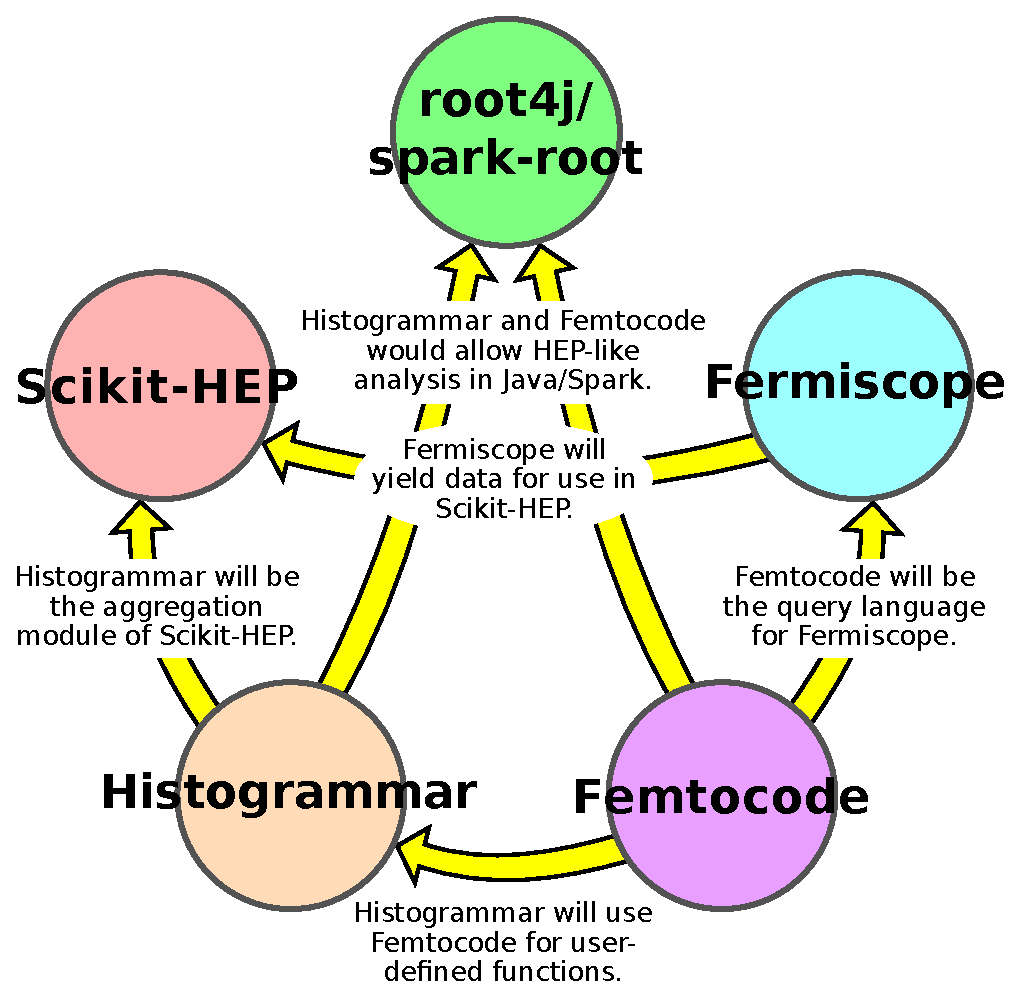
\includegraphics[width=0.8\linewidth]{relationships.pdf}
\end{center}
\end{frame}

\begin{frame}{Meta-strategy}
\vspace{0.25 cm}
\begin{itemize}
\item Diverse suite of projects with interconnections:
\begin{itemize}
\item Not everything has to work, but they're all better if they do.
\item If a competitor succeeds in some area, don't fight them. Concentrate on the others while the connection to successful projects provides an implicit incentive to grow later.
\end{itemize}

\item Focusing on building developer communities before user communities.
\begin{itemize}
\item Aiming for 1--2 users of each project once it's minimally useful, then broadening to a wider user base when it's stable.
\item But I'm trying to bring in as many developers as there are use-cases. Each concentrates on his/her direct need.
\item This includes developers outside of HEP, if possible.
\item Planning on using focus groups of users to guide design, rather than just reacting with release-early-release-often.
\end{itemize}
\end{itemize}
\end{frame}

\begin{frame}{Detailed descriptions: Histogrammar}
\vspace{0.6 cm}
\begin{columns}
\column{0.4\linewidth}
Aggregate data from a variety of backends, plot it in a variety of frontends.
\column{0.5\linewidth}

\includegraphics[width=\linewidth]{histogrammar-logo.png}
\end{columns}

\vspace{0.4 cm}
Composable aggregators that are good for parallelization, particularly good for functional frameworks like Spark, as well as conceptual and performance advantages for PyROOT.

\vspace{0.4 cm}
\textcolor{darkblue}{Status:}
\begin{itemize}
\item Successful beta-tester stage; user-ready but adoption is slow.
\item Introduced to physicists in many one-on-one sessions, to industry in high-profile talks. Everyone was excited while we talked, but few followed up.
\item Missed ROOT release because ROOT wasn't ready to include Python subpackages. Will target Scikit-HEP instead. \\ \textcolor{gray}{(And possibly add a C++ Histogrammar to Enrico Guiraud's or Brian's functional chains.)}
\end{itemize}
\end{frame}

\begin{frame}{Detailed descriptions: Scikit-HEP}
\vspace{0.5 cm}
\begin{columns}
\column{0.6\linewidth}
rootpy, root\_numpy, and Ostap are widely-used Pythonic layers for ROOT.

\vspace{0.2 cm}
I suggested combination into a single project to build on existing momentum, but I probably won't be a major contributor \textcolor{gray}{(except for Histogrammar)}.

\vspace{0.2 cm}
Also shifting focus from ``Python and ROOT'' to ``Python and HEP.''
\column{0.3\linewidth}
\scriptsize

\includegraphics[width=\linewidth]{femtocode-logo.png}

\textcolor{darkgray}{Note: logo suggestion has not been agreed upon.}
\end{columns}

\vspace{0.4 cm}
\textcolor{darkblue}{Status:}
\begin{itemize}
\item Everyone's enthusiastic and we discuss progress in regular meetings by Skype and Slack.
\item Mostly refactoring/relicensing the original projects, preparing for the big merger.
\item I'm beginning to advertise it (Wednesday's LPC Coffee Chat).
\end{itemize}
\end{frame}

\begin{frame}{Detailed descriptions: root4j/spark-root}
\vspace{0.5 cm}
Follow-up to my early work this year converting ROOT to Avro for Oli \& Matteo's analysis and replaces earlier plans of connecting ROOT to Apache Arrow.

\vspace{0.3 cm}
\begin{columns}[t]
\column{0.45\linewidth}
\mbox{ } \hfill \underline{File conversion} \hfill \mbox{ }

\vspace{0.1 cm}
Makes the bookkeeping problem worse, defeating the main benefit of Spark.

\column{0.45\linewidth}
\mbox{ } \hfill \underline{Direct reading} \hfill \mbox{ }

\vspace{0.1 cm}
C++ ROOT via JNI is buggy, but the old pure-Java package works (with a little effort).
\end{columns}

\vspace{0.4 cm}
\textcolor{darkblue}{Status:}
\begin{itemize}
\item Viktor Khristenko has completely taken over the codebase, and is actively using it on his own thesis. I just need to make sure it works for other use-cases.
\item Directly juxtaposed with Danilo \& Enric (ROOT Team)'s ROOT-in-Spark. Trying to apply both to the same use-case: Marc Dunser (CMS). Having trouble getting Marc's attention.
\end{itemize}
\end{frame}

\begin{frame}{Detailed descriptions: Femtocode}
\vspace{0.5 cm}
I've been thinking about a more abstract numerical language (an ``executable chalkboard'') for a long time. See my earlier \href{http://dmg.org/pfa/}{\textcolor{blue}{PFA}}.

\vspace{0.3 cm}
After months of talking about it, gauging interest and prior art (inside and outside of HEP), I've found a niche that really needs it: big data pulls. See \href{https://indico.cern.ch/event/594180/}{\textcolor{blue}{Monday's talk}}.

\vspace{0.4 cm}
\textcolor{darkblue}{Status:}
\begin{itemize}
\item Started implementing, off and on, right after CHEP in October. Progress is pretty good, considering.
\item I'm finding it hard to describe what Femtocode is and what it's about.
\item Peter Hansen has signed on to write the GPU backend, but interactions have been slow. \textcolor{gray}{(Femtocode doesn't strictly need a GPU backend, though I think it would be a great target.)}
\end{itemize}
\end{frame}

\begin{frame}{Detailed descriptions: Fermiscope}
\vspace{0.4 cm}
Early on, I thought HEP needed an Ibis/Impala/Kudu/Drill-type thing to make plots in seconds, rather than private skims in weeks. Oli's interest in Spark won out.

\vspace{0.3 cm}
Using Spark's DataFrames, I came to realize that the optimization these systems provide wouldn't be available to non-flat ntuple analysis without Femtocode-like extensions.

\vspace{0.3 cm}
Meshed with Jin \& Igor's NoSQL LDRD project by convergence. Now they'll need Femtocode with a Sep.\ 2018 final due date.

\vspace{0.4 cm}
\textcolor{darkblue}{Status:}
\begin{itemize}
\item It's hard for Igor to do much without minimally working Femtocode, but we've been converging on the shape of the project. Progress picked up this week.
\item Using off-the-shelf parts wherever possible: CouchBase for storage, possibly Charm++ for execution.
\end{itemize}
\end{frame}

\begin{frame}{Conclusions}
\vspace{0.5 cm}
\textcolor{darkblue}{Overall goal: widely used code and some publications.}

\vspace{0.25 cm}
Not much to show yet:

\begin{itemize}
\item Histogrammar adoption should be higher than it is.
\begin{itemize}
\item I did spend time evangelizing it, to the detriment of other work.
\item Response has been excitement without application.
\item It will be important in later projects (Femtocode, Fermiscope), so it's not a loss to set it aside for a while.
\end{itemize}

\item All other projects are too early to judge.

\item Missed the first round of HEP-computing conference deadlines because they're early in the year and I wasn't ready back then. Gearing up for next year's cycle.
\begin{itemize}
\item On Nan Niu (Cincinnati)'s suggestion, I'm going to submit my work on focus groups to the \href{http://se4science.org/workshops/}{\textcolor{blue}{SE4Science Workshop}}.
\item Will be working with Brian on a ``languages for HEP'' white paper; haven't started.
\item But main publications should be on the projects described here.
\end{itemize}
\end{itemize}
\end{frame}

\end{document}
